\documentclass[border=2pt,tikz]{standalone}
\usepackage{tikz}
\usepackage{amsmath}
\usepackage{amssymb}

\begin{document}

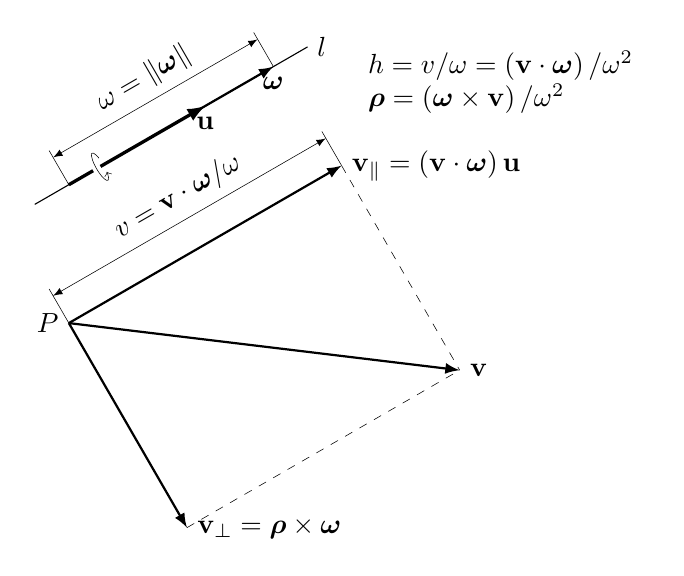
\begin{tikzpicture}

\begin{scope} [yshift=50.0, rotate=30]

\draw[thin] (-0.5,0.0) -- (3.5,0.0) node [right] {$l$};
\draw[very thick,->,>=latex] ( 0.0,0.0) -- (2.0,0.0) node [below] {$\mathbf{u}$};
\draw[thick,->,>=latex] ( 1.80,0.0) -- (3.0,0.0) node [below] {$\boldsymbol{\omega}$};

\draw[very thin] (0.0,0.0) -- (0.0,0.5);
\draw[very thin] (3.0,0.0) -- (3.0,0.5);
\draw[very thin,<->,>=latex] (0.0,0.4) -- node [above, rotate=30] {$\omega=\left\Vert \boldsymbol{\omega}\right\Vert $} (3.0,0.4);
\draw[color=white,line width=3] ( 0.41,0.1) -- (0.41,-0.1);
\draw[very thin, ->] (0.50,0.10) arc (30:330:0.05 and 0.20);

\end{scope}

\begin{scope} [rotate=30]

\draw[thick,->,>=latex] ( 0.0,0.0) -- (4.0, 0.0) node [right] {$\mathbf{v}_\parallel = \left(\mathbf{v} \cdot \boldsymbol{\omega}\right)\mathbf{u}$};
\draw[thick,->,>=latex] ( 0.0,0.0) -- (0.0,-3.0) node [right] {$\mathbf{v}_\perp=\boldsymbol{\rho} \times \boldsymbol{\omega}$};
\draw[thick,->,>=latex] ( 0.0,0.0) node [left] {$P$} -- (4.0,-3.0) node [right] {$\mathbf{v}$};
%\draw[very thick,->,>=latex] ( 0.0,0.0) -- (2.0,0.0) node [below] {$\mathbf{u}$};

\draw[very thin] (0.0, 0.0) -- (0.0,0.5) ;
\draw[very thin] (4.0, 0.0) -- (4.0,0.5) ;
\draw[very thin,<->,>=latex] (0.0, 0.4) -- node [above, rotate=30] {$v=\mathbf{v} \cdot \boldsymbol{\omega} / \omega$} (4.0,0.4) ;

\draw[very thin,dashed] (4.0, 0.0) -- (4.0,-3.0) ;
\draw[very thin,dashed] (0.0,-3.0) -- (4.0,-3.0) ;

\end{scope}

\node[above right] at (3.5, 2.5) {$\begin{array}{l}
h=v/\omega=\left(\mathbf{v} \cdot \boldsymbol{\omega}\right)/\omega^{2}\\
\boldsymbol{\rho}=\left(\boldsymbol{\omega}\times\mathbf{v}\right)/\omega^{2}
\end{array}$};

\end{tikzpicture}

\end{document}

